\documentclass[12pt]{scrartcl}
\usepackage{graphicx}
\usepackage{amsmath}

\begin{document}

%Title section

\titlehead{CS department, Technion}
\subject{Introduction to Optimization and Deep Learning 236330}
\title{HW 3}
\subtitle{Quasi-Newton BFGS method and DNN training}
\author{Uri Kirstein 311137095 \hfill sukirstn@campus.technion.ac.il\and Pavel Rastopchin 321082026 pavelr@campus.technion.ac.il}
\date{\today}
\maketitle

 %end of title section
\section*{Part 1 - BFGS}
\subsection*{Task 2}
We chose $N=10$. Our starting point was $x_0=(0,0,..0)$. We know that a local minimum of the function exists at $x^*=(1,1,...)$ and that $p^*=0$ (our function is non-negative so this must be a global minimum as well). We stopped after 97 iterations at\\\\
$x_{final}$=[ 5.51033772e-07,  6.67959021e-07, -4.45033926e-06, 
2.72106755e-06, 1.86952265e-06, -7.31025632e-09, -1.21113396e-06, -5.86666139e-06, 4.51107833e-06, -5.76553427e-07]\\\\
The error function and gradient at this point are $$f(x_{final})-p^*=5.359357003868173e-14$$
$\nabla f(x_{final})=$[ 5.51033772e-07  6.67959021e-07 -4.45033926e-06  2.72106755e-06\\
  1.86952265e-06 -7.31025632e-09 -1.21113396e-06 -5.86666139e-06
  4.51107833e-06\\ -5.76553427e-07]
$$||\nabla f(x_{final})|| = 9.381977770909129e-06$$
We can see in the graph below that the error function $f(x_k)-p^*$, where $k$ is the number of iterations, is monotonously decreasing. This means we always advance in the direction of the minimum.
\begin{figure}[h!]
	\hfill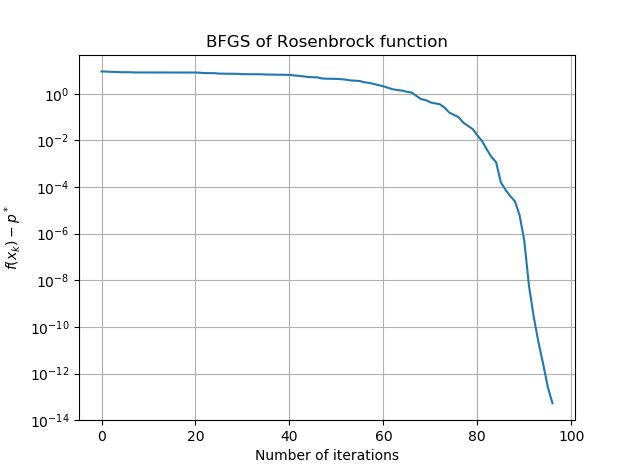
\includegraphics[width=\linewidth]{rosenbrock_graph.jpg}\hspace*{\fill}
	\caption{Task 2}
\end{figure}

\end{document}
